\chapter{Methodology}

In this chapter it is going to be explained all the steps required to achieve a functional neural network to participate at the ActivityNet Challenge. For this challenge there was no baseline because video tasks have not been faced on the group I did this project, so was required to face the challenge from scratch.

\section{Objective}

For this project, the aim has been to obtain a Neural Network capable of classify and temporally localize activities and videos. In order to get that, the proposal is, once the features has been extracted with the C3D, predict with a RNN a sequence of activities that might be happening for every 16-frame clip. So as the output of the Neural Network, is expected to have a sequence each item giving the activity happening at each video clip as input. This approach offers more advantages that others being able to classify the whole video and even localize along the video sequence them multiple activities happening and their temporal localization.
\section{ActivityNet Dataset}

The ActivityNet Dataset\cite{caba2015activitynet} is \textit{A Large-Scale Video Benchmark for
Human Activity Understanding}. This dataset, on version 1.3 which is the one used for the challenge, contains 19,994 videos with a different 200 activities labeled which represents a wide range of human activities. In total there are 660 hours of video and the subsets are split on the following way: 50\% training dataset, 25\% validation dataset and 25\% testing dataset. Each video of the dataset have an activity happening in there and one or more annotations saying in which temporal locations the activity is happening.

The dataset was provided as a description file, which the URL of the video was provided and also the ground truth annotations for the training and validation subset as a set of starting time, ending time and the activity happening between the given interval. In addition more information was given such as the original video resolution and the duration.

Because all the video from this dataset are placed on \textit{YouTube} so only the links for the video are provided because of copyright issues. So the first task to be done was download all the videos on our own. This was done using a program called \textit{youtube-dl} which allows to download videos from that platform. But some videos show up with some issues as all of them were stored on a third party platform. This issues went from some of them presenting location restrictions to some of them  even were removed by their owners. This let only download 19,811 video which considering the size of the dataset, was not a big deal.

Once all the videos from the dataset were downloaded, the number of frames of each video was extracted because the temporal unit at the time to process it will be the frames. It was decided to use all the frames that each video has to fed the feature extraction and because of this, the temporal resolution in order to predict the activities happening along the video may vary between 0.5 and 1 second of resolution.

In addition to this, some stats were computed. Such as the whole number of frames from all the videos in the dataset which is 65.6 million frames. Also, the length in minutes of each activity at the dataset was plot on Figure~\ref{fig:dataset_stats} to have an idea about the activities frequencies. As can be seen, not all the activities have the same appearance along the dataset, varying from 40 minutes the least frequent activity to 3.5 hours the more frequent one. In total over all the dataset there are 313 hours of activities which will be required to detect and localize.

\begin{figure}[H]
\begin{center}
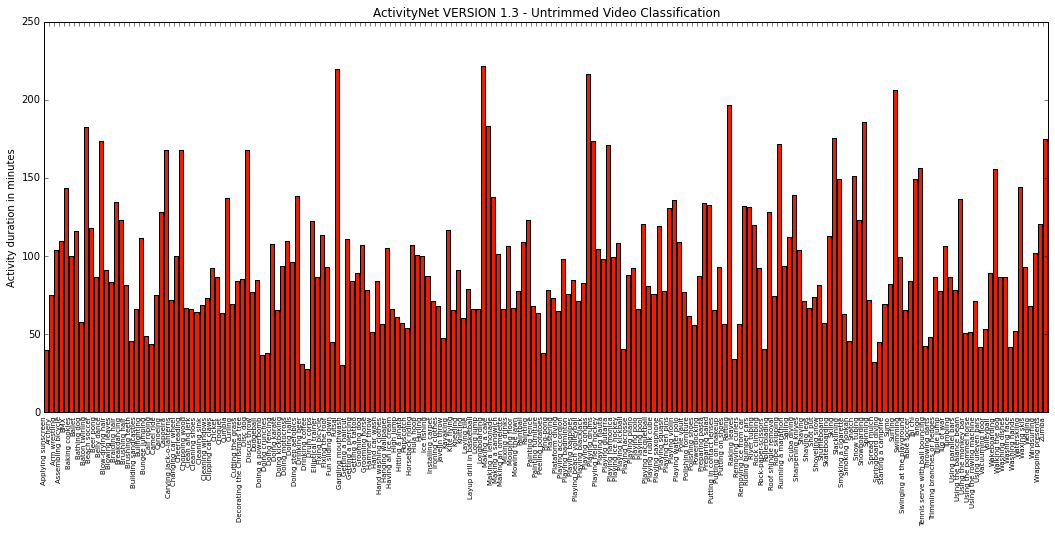
\includegraphics[width=1\linewidth]{img/methodology/dataset_stats}
\end{center}
\caption{Activity duration in minutes for each activity on the dataset}
\label{fig:dataset_stats}
\end{figure}

\section{Extracting Video Features Using C3D}

The C3D network\cite{tran2014learning} was decided to use as a video features extractor to be known to extract very well\cite{baccouche2011sequential}\cite{tran2015deep}\cite{tran2014learning}\cite{shoutemporal} either spatial and temporal correlations from videos. This network is made up of 8 convolutional layers, plus 5 pooling layers and 2 fully-connected layers at the end. The convolutional layers have $3 \times 3 \times 3$\footnote{For notation, the dimension ordering is $d \times k \times k$ where $d$ is temporal dimension and $k$ is spatial dimension} kernels and stride 1 while at the same time the pooling layers compute the maximum at every kernel size of $2 \times 2 \times 2$ except from the first pool layer which has a $1 \times 2 \times 2$ kernel size. On the Figure~\ref{fig:c3d_architecture} there is the representation of the C3D architecture with the number of kernels or neurons of each convolutional layer and fully-connected layer.
%%TODO add references

\begin{figure}[H]
\begin{center}
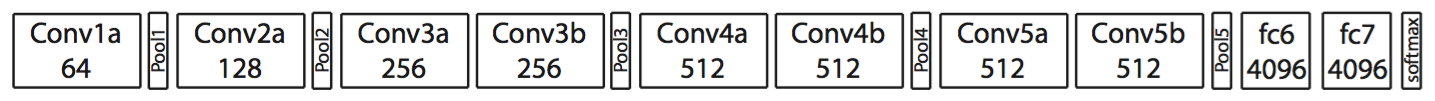
\includegraphics[width=1\linewidth]{img/methodology/c3d_architecture}
\end{center}
\caption{Architecture of the C3D network}
\label{fig:c3d_architecture}
\end{figure}

The original paper proposing and studying 3D convolutions applied to videos, also give code to reproduce it. The code given was based on a version of \textit{Caffe}\cite{jia2014caffe} dated to 2014. Because the code to use 3D convolutions did not support last features and did not work with the \textit{Python} environment used for this project, the model trained with C3D and the Sports1M\cite{KarpathyCVPR14} dataset was ported to \textit{Keras}\footnote{All the process has been open sourced and can be found in: \url{https://gist.github.com/albertomontesg/d8b21a179c1e6cca0480ebdf292c34d2}}. Keras is a deep learning framework that works over \textit{Theano}\cite{theano2016theano} and \textit{TensorFlow}\cite{abadi2016tensorflow}, two computational frameworks which allow run and train deep learning models over either CPU and GPU. For this work, \textit{Theano} was used as back-end to do the computations because their support for 3D convolutions operations.

At the time to run the C3D model on the model ported to \textit{Keras}, some little changes where required to do over the source code\footnote{The fork of \textit{Keras} used can be found in: \url{https://github.com/albertomontesg/keras/tree/develop}} due to the implementation of the 3D convolution and 3D pooling operations. Once this was fixed, all the videos where passed through the C3D model, and its features at \textit{fc6} extracted. This process could be done in parallel with 2 GPUs computing the features and multiple CPU cores fetching from disk all the videos. This task was expected to last a lot of time (one week approximately) but thanks to parallelize the process, only in two days all the features where computed from the 65.6 million frames available at the dataset.

In the process of fetching the videos from disk, was used \textit{OpenCV}\cite{opencv_library} a framework with interesting utils for Computer Vision applications. With this software, the videos were read in chunks of 16 frames, resized to 112x112 as input frame size and then feed the C3D network. The output of the model, a sequence of 4096-sized vectors where stored in disk for preparing it to train the Recurrent Neural Network.

\section{Extracting Audio Features}

The audio features extracted: MFCC and Spectral

I require to ask Ignasi for references. How much importance I have to make to the audio features. At the results adding audio features does not improve the results with only the video features.

%%TODO: Ask for bibliography

\section{Prepare the Data for Stateful Recurrent Networks}

Since all the videos on the ActivityNet Dataset are not from the same length, to train a recurrent neural network, it requires to give it a fixed length sequence. This length is called \textit{timestep} and must be a value not very high because as the gradient propagates along all the sequence, if the timestep is very high, the gradient might achieve very high values known as \textit{exploiting gradient}.

There are two main solutions to this, in order to keep the memory state of the LSTM cells for a long sequences. The first solution would require to clip it as is explained in \cite{pascanu2012difficulty}. The second solution is to train the Recurrent Neural Network without resetting the memory between each batch. With this approach, if a video sequence longer than the \textit{timestep} does not fit into the batch, the RNN can be trained passing fragments of the videos as clips one after the other at the same batch position, and because the memory is not reset after each batch, at the training of the next batch, the memory will be preserve. For this configuration the different videos must be carefully set on the same batch index to exploit the \textit{Keras} functionality of stateful training for RNNs.

\begin{figure}[H]
\begin{center}
\includegraphics[width=1\linewidth]{img/methodology/stateful_dataset}
\end{center}
\caption{Graphical representation of how the data is sorted in order to train RNNs}
\label{fig:stateful_dataset}
\end{figure}

In the Figure~\ref{fig:stateful_dataset} is graphically represented how the video features are organized to train the Recurrent Neural Network. The notation for the data is as follows, where $\bar{X}$ is the feature vector of a 16 frame clip extracted from the C3D network, and $V_i$ the sequence of features for a single video. Note that $T_i$ is the length of the sequence of each video $i$ in number of 16-frame clips.

\begin{equation}
	\bar{X} = [x_i, x_2, \ldots, x_{4096}]
\end{equation}
\begin{equation}
	V_i = \{ \bar{X}_t \}_{t=1}^{T_i}
\end{equation}

In order to try to fit the most possible data into the GPUs when training each batch and to get a good gradient propagation along the batch's sequence length, for all the experiments done on this project, the batch size was 256 and the timesteps 20.

As the last step to prepare the data, the output information was computed for each 16-frame clip as follows: if the Intersection Over Union (IOU) between the temporal range of the 16-frame clip and the ground truth annotations was higher than $0.5$, the clip was cataloged as the activity of the ground truth annotation. If the IOU was lower, it was cataloged as background activity. So at the training and validation subsets, the output was encoded with the one-hot encoding, which puts a 1 at the position of the class given and 0s on the rest. This way to encode the output is the used for Softmax output layers which represent the probability of each class to be predicted as the output is between 0 and 1.

\section{Networks Configuration}

So as to achieve the aim of this project, which is to find a good Neural Network which is capable of classify activities and detect its temporal location in videos, the Recurrent Neural Networks were decided to be used with LSTM which have been demonstrated to learn from long term correlations. The RNN had the inputs and output previously explained, and so an experimentation of the architecture was done. 

The basic architecture consist in a single layer of LSTM with 512 cells which end-up with a total of 9.5 millions parameters. From this network as a basic one, on this project there has been some experimentation trying with more deep networks with even more cells. On Figure~\ref{fig:lstm_architecture} there is represented the network architecture.

\begin{figure}[H]
\centering
\begin{subfigure}[b]{.5\textwidth}
  \centering
  \includegraphics[width=1\linewidth]{img/methodology/lstm_architecture_basic}
\end{subfigure}%
\begin{subfigure}[b]{.5\textwidth}
  \centering
  \includegraphics[width=1\linewidth]{img/methodology/lstm_architecture_deep}
\end{subfigure}
\caption{Architecture of RNN used with 512-LSTMs with one and two layers respectively.}
\label{fig:lstm_architecture}
\end{figure}

With the basic architecture was observed that the activity prediction, in some cases was very different in short periods of time, predicting between two activities or one activity and the background class. To solve this problem, another architecture proposed consist in the previous basic one, but with an additional input at the bottom which consist the previous output of the sequence. This kind of feedback, was expected to give more smooth predictions as the network is aware about which was exactly the previous activity predicted.

For this network, a new input was added to the video features which was the one-hot encoding of the previous output with an added value, which will be always zero except to the first video feature, which do not have previous output, and will be marked with a one. With this extra value, is expected that the network learn to forget its memory state because the begging of a video sequence. In the Figure~\ref{fig:lstm_architecture_feedback} can be found the architecture previously explained with feedback.

\begin{figure}[H]
\begin{center}
\includegraphics[width=0.6\linewidth]{img/methodology/lstm_architecture_feedback}
\end{center}
\caption{Architecture of the RNN network with feedback from the previous output}
\label{fig:lstm_architecture_feedback}
\end{figure}



%%%%% Talk about semisupervised training???????



\section{Training}

At the time to train, some parameters required to be specified, and some problems appear with them. For training a loss function was chosen, also known as objective function. For the configuration proposed, the best loss function to choose is the categorical cross entropy because the use of Softmax as output which predicts each activity probability and can be considered as a probability distribution. It is computed as follows,

\begin{equation}
	H(p,q) = - \sum_x p(x) \log(q(x))
\end{equation}

where $q$ is the predicted probability distribution and $p$ the ground truth probability distribution.

Another important parameter to setup for training is the optimizer function. For training Recurrent Neural Networks, the best choice is to use the RMSprop\cite{dauphin2015rmsprop} with a value of $\rho$ of 0.9 and $\epsilon$ of $10^{-8}$. The learning rate, otherwise, have been the value that has need to be tuned. At the training, starting with high values for the learning rate, it was observed that the network did not learned and the validation loss increased instead of decreasing. On the Figure~\ref{fig:training_curves_comparison} can be seen the difference between training the same network with a different values of learning rate. Finally the best learning rate that was found to work better at the time to train is $10^{-5}$.

\begin{figure}[H]
\centering
\begin{subfigure}[b]{.5\textwidth}
  \centering
  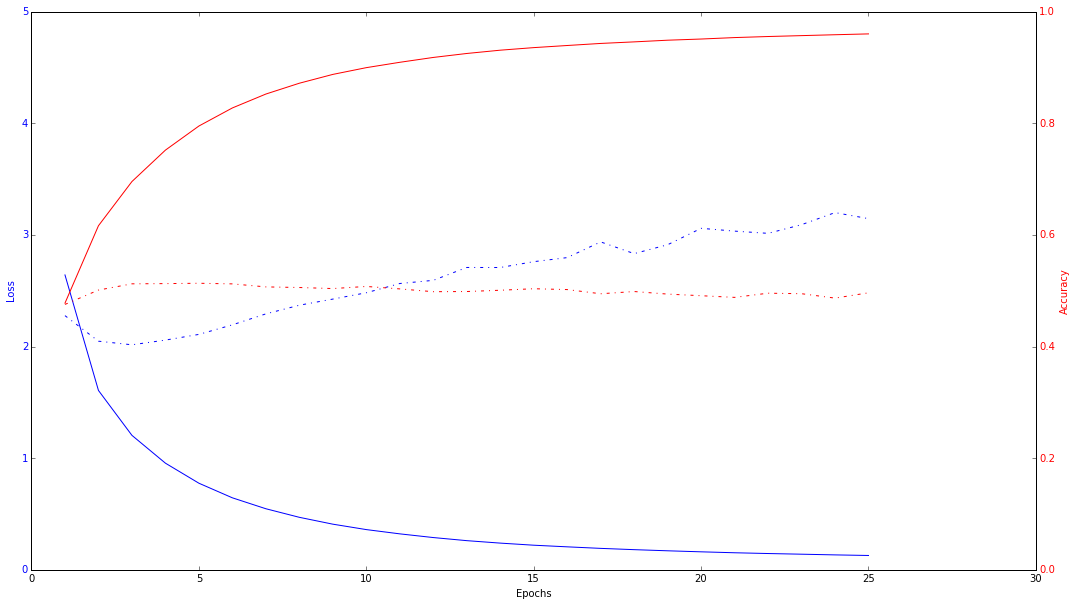
\includegraphics[width=1\linewidth]{img/methodology/training_bad}
\end{subfigure}%
\begin{subfigure}[b]{.5\textwidth}
  \centering
  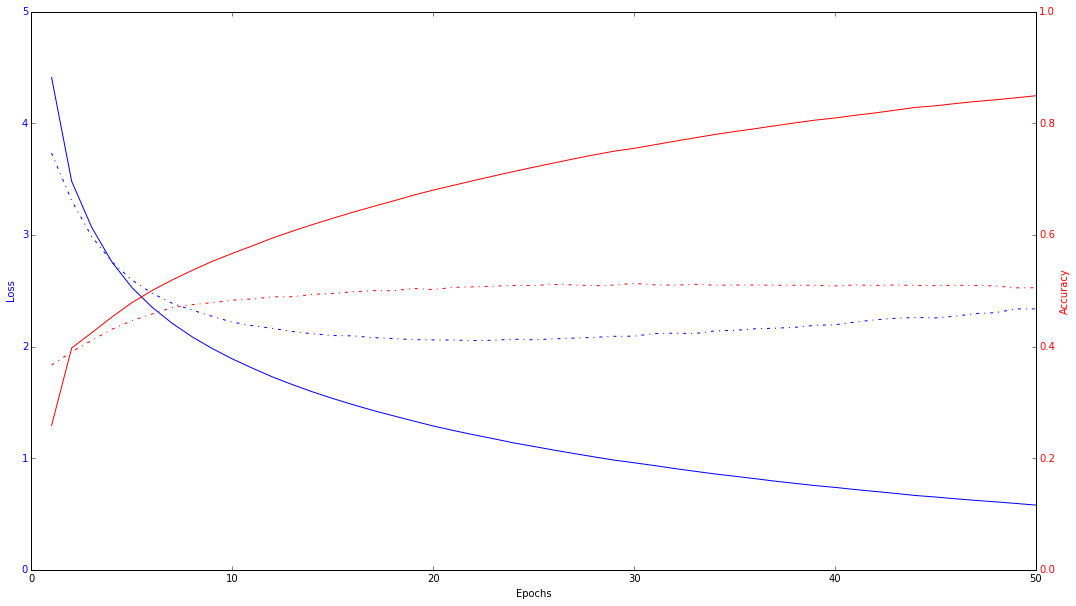
\includegraphics[width=1\linewidth]{img/methodology/training_good}
\end{subfigure}
\caption{Comparison of the learning curves. On the left with a learning of $10^{-4}$ and at the right figure with a learning rate of $10^{-5}$}
\label{fig:training_curves_comparison}
\end{figure}

In addition to find the right value for the learning rate, some other problems appear. Even with a good learning rate to learn, it was observed that the network presented some over-fitting due mostly to the high learning capacity the network has over the data. So, in order to fix that, dropout\cite{srivastava2014dropout} layers were added before and after the LSTM layers to reduce this over-fitting. Dropout consists in randomly setting a fraction $p$ of input units to 0 at each update during training time. The value of $p$ chosen was 0.5.

Another inconvenience found during training, was related to the fact of having as an input multiple vectors from multiple sources. When training with the visual features extracted from the C3D network, with the audio features or/and the previous output, as all of them presented a different statistics, a normalization was required. So for all the experiments, a batch normalization\cite{ioffe2015batch} was placed after the input data in order to have all the inputs with the same statistics, mean 0 and standard deviation equal to 1. 

The last problem that was necessary to face, was related with the fact of unbalanced output. All the activities had the approximately the same frequency of appearance, but nearly half of the video clips correspond to a non-activity, or as it has been defined, background class. So with this huge unbalance of the output classes, it was decided to weight the loss function in order to slow down the learning when the background class was predicted. With this method the predicted output will not be so bias towards the background class.

The new loss function taking into account the unbalanced classes is

\begin{equation}
	H(p,q) = \sum_x \alpha(x) p(x) \log (q(x)), \text{ where } \alpha(x) = 
    \begin{cases}
        \rho, & x = \text{background instance}\\
        1,    & \text{otherwise}
    \end{cases}
\end{equation}

where $\rho$ is the factor used to weight the loss for background instances at training. This value $\rho$ is usually computed as 1 minus the frequency of appearance of the class (for all the activities class can be simplified to 1). For the background class was found the its frequency of appearance was 0.4 so it was tested to setup $\rho = 0.6$. The results did present a little improvement so it was decided to even do smaller this value, setting it finally $\rho = 0.3$.

\section{Post-Processing Proposed}
\label{section:post_processing}

The network proposed gives as an output the predicted activity probability for each 16-frames clip. For the challenge to face during this project, and for the aim of this project is required to compute from the output obtained the activity classification for the whole video and the temporal localization of this activity. To obtain this information, some post-processing was required as it is not directly predicted from the network.

\subsection{Classification Task}

For the classification task, what was done as the first stage was remove the output probability corresponding to the background class and normalize the rest of the activities probabilities (the sum of all the probabilities for each clip become to be 1). Once the background class was removed (as it is known that in all of the videos in the ActivityNet Dataset, there is one activity on it), then the mean of each video activity class was computed along the video's output sequence.

\begin{equation}
	p_{video}(x) = \frac{1}{T_{video}} \sum_i^{video} p_i(x), \text{where } x \in \{ \text{Dataset Activities}\}
\end{equation}

With this operation, there is for each video in the dataset a vector of probabilities, each one giving the probability of each activity happening along the video. All the values given by this vector where the ones used to make the prediction, taking the activity highest probable as the video activity and the probability of prediction computed as the score.

\subsection{Detection Task}
 
For the detection task of the ActivityNet Challenge, or temporal activity localization, more operations were required in order to predict temporal annotations on the temporal dimension. As is known that at every video of the ActivityNet Dataset all the annotation are of the same activity, the classification activity was first computed and give it as solution for all the temporal localization.

Working with the sequence probabilities predicted by the Neural Network, a mean filter was applied. This mean filter has a parameter $k$ which represent the number of clips behind and forward that delimiter the window to compute the mean. The way to compute it is described on Equation~\ref{eq:mean_filter}. Applying this filter, it has been achieved a more smooth output prediction and better results.

\begin{equation}
	\tilde{p}_i(x) = \frac{1}{2k} \sum_{j=i-k}^{i+k} p_i(x)
    \label{eq:mean_filter}
\end{equation}

The next step was compute the activity probability as the sum of all the output classes except the background class.
\begin{equation}
	\tilde{p}^a_i = \sum_{x=1}^{200}\tilde{p}_i(x), \text{where } x = \begin{cases}
        0, & \text{background class} \\
        i, & 1 \leq i \leq 200 \text{ activity classes}
    \end{cases}
\end{equation}

Once is known the probability of having an activity for each clip of the video, a threshold~$\gamma$ has been defined. In order to localize temporally the activities along the video, the annotations finally given by the post-processing will be the temporal sequences of the video which has a higher activity probability $\tilde{p}^a_i$ higher than the threshold $\gamma$. Playing with the values of $k$ of the mean filter and the threshold $\gamma$ it has been possible to find the best values to get the best performance. The results of all the experimentation described on this section is detailed on Section~\ref{section:results}

